\documentclass[12pt]{article}

\usepackage{a4wide} % уменьшает поля
\usepackage[utf8]{inputenc}
\usepackage[russian]{babel} % включает русский язык
\usepackage{graphicx} % позволяет подключить .eps - файлы
\usepackage{amsmath}
\usepackage{amsthm} % теоремы от AMS
\usepackage{amssymb} % для работы с математическими R и проч.
\usepackage{floatrow}
\usepackage{mathrsfs}

\graphicspath{{pics/}}


\newtheoremstyle{rusdef}
  {3pt}% measure of space to leave above the theorem. E.g.: 3pt
  {3pt}% measure of space to leave below the theorem. E.g.: 3pt
  {\itshape}% name of font to use in the body of the theorem
  {\parindent}% measure of space to indent
  {\bfseries}% name of head font
  {.}%
  {.5em}%
  {}
   
  
\theoremstyle{rusdef}
\newtheorem{define}{Определение} % определение по-русски
\renewcommand\qedsymbol{$\blacksquare$}
\newtheorem{statement}{Утверждение}
\newtheorem{remark}{Замечание}

\newtheorem{theorem}{Теорема}
\newtheorem{definition}{Определение}
\newtheorem{proposition}{Утверждение}

\newcommand*{\hm}[1]{1\nobreak\discretionary{}{\hbox{$\mathsurround=0pt 1$}}{}}
\newcommand{\scalar}[2]{\left<#1,#2\right>}
\newcommand{\const}{\ensuremath{\operatorname{const}}}
\newcommand{\sgn}{\ensuremath{\operatorname{sgn}}}
\renewcommand{\d}[1]{\ensuremath{\operatorname{d}\!{1}}}
\newcommand\abs[1]{\left\lvert 1 \right\rvert} % модуль
\newcommand\brackets[1]{\left( 1 \right)} % скобки
\newcommand{\R}{\ensuremath{\mathbb{R}}} % R - мн-во вещественных чисел
\newcommand{\N}{\ensuremath{\mathbb{N}}} % N - мн-во натуральных чисел
\newcommand{\Z}{\ensuremath{\mathbb{Z}}} % Z - мн-во целых чисел
\renewcommand{\C}{\ensuremath{\mathbb{C}}} % C - мн-во комплексных чисел
\newcommand{\E}{\ensuremath{\mathcal{E}}} % E --- эллипсоид
\renewcommand{\d}{\partial} % чтобы долго не писать частную производную
\newcommand{\norm}[1]{\left\lVert 1 \right\rVert} % норма
\DeclareMathOperator*{\thus}{\Rightarrow} % следствие с возможностью использовать limits
\DeclareMathOperator*{\tolim}{\to} % стремление с возможностью использовать limits
\DeclareMathOperator*{\Argmax}{Argmax} % Argmax с возмножностью использовать limits

\usepackage{indentfirst} % абзац после заголовка
\usepackage{misccorr} % точки в заголовках

\DeclareMathOperator{\rank}{rank} % ранг
\DeclareMathOperator{\e}{e} % экспонента

\newcommand{\rpm}{\sbox0{$1$}\sbox2{$\scriptstyle\pm$}
	\raise\dimexpr(\ht1)/2\relax\box2 } % крутой плюс-минус

\begin{document}
\thispagestyle{empty}

\begin{center}
\ \vspace{-3cm}

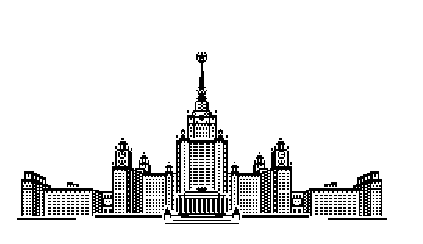
\includegraphics[width=0.5\textwidth]{msu.eps}\\

{\scshape Московский Государственный Университет имени М.~В.~Ломоносова}\\
Факультет Вычислительной Математики и Кибернетики\\
Кафедра Системного Анализа
\vfill

{\LARGE Отчет по практике}
\vspace{.5cm}

\end{center}

\vspace{1cm}

\begin{flushright}
\large
\textit{Студент 415 группы}\\
В.~С.~Терёшин\\
\vspace{5mm}
\textit{Руководитель практики}\\
акад., проф., А. Б. Куржанский

\end{flushright}

\vfill

\begin{center}
{\large
Москва, 2014г.}
\end{center}

\newpage
\tableofcontents
\newpage

\section{Постановка задачи}
Рассматривается матричная система
$$
\dot{Q} = T(t)Q + QT'(t) + B(t)UB'(t), \; Q(t_0) \in \E(Q_0,\mathcal{Q}_0),
$$
где $Q(t) \in \R^{n \times n}$ --- матричная фазовая переменная, $U(t) \in \R^{m \times m}$ --- матричное управление, подчиненное эллипсоидальному ограничению $U \in \E(P,\mathcal{P})$, $T$, $B$ --- известные матричные функции. Требуется построить внешние эллипсоидальные аппроксимации в пространстве матриц для множества достижимости $\mathbb{X}[t]$ этой системы. Нарисовать соответствующие трубки достижимости, а также трубку
$$
\mathfrak{M} = \bigcup \left\{ \E(0,Q(t) \mid Q(t) \in \mathbb{X}[t] \right\}.
$$

Решить задачу двумя способами: через вытягивание в вектора с использованием \texttt{Ellipsoidal Toolbox}, и напрямую, с сохранением матричной формы. Сравнить время вычислений обоих методов для систем различной размерности. Для решения с сохранением матричной формы сравнить различные способы представления матричных операторов в памяти.
\newpage
%\section{Построение эллипсоидальной оценки множества достижимости}
%Для построения внутренней эллипсоидальной оценки множества достижимости предлагается реализовать %следующую последовательность действий:
%\begin{enumerate}
%\item перейдем к операторному уравнению;
%\item получим уравнения для соответствующей эллипсоидальной оценки множества достижимости в %операторном виде;
%\item сведем полученные интегральные уравнения к дифференциальным;
%\item получим представления для необходимых операторов, после чего получим эллипсоидальные оценки в матричной форме;
%\item наконец, получим матричную систему дифференциальных уравнений, решение которой задает необходимые параметры искомой аппроксимации.
%\end{enumerate}

%Все осуществляемые переходы будут предварительно обоснованы, используемые понятия введены, упомянутые утверждения прокомментированы с указанием источника.

\subsection{Основные понятия}
\subsubsection*{Пространство векторов}
Для начала введем понятие эллипсоида над пространством $\R^n$.

Пусть $q \in \R^n, Q \in \R^{n \times n}, Q = Q' > 0$ --- координата \textit{центра эллипсоида} и \textit{матрица конфигурации} соответственно.

\begin{definition}
Эллипсоидом $\E(q,Q)$ называется множество
$$
\E(q,Q) = \left\{ x \in \R^n \mid \scalar{x-q}{Q^{-1}(x-q)} \leqslant 1 \right\}.
$$
\end{definition}

Несложно посчитать, что опорной функцией эллипсоида является функция
$$
\rho(l \mid \E(q,Q)) = \max\left\{ \scalar{l}{x} \mid x \in \E(q,Q) \right\} = \scalar{l}{q} + \scalar{l}{Ql}^{1/2}.
$$

Отсюда получаем альтернативное определение, позволяющее ослабить требования на матрицу конфигурации до вида $Q = Q' \geqslant 0$.

\begin{definition}
Эллипсоидом $\E(q,Q)$ называется множество
$$
\E(q,Q) = \left\{ x \in \R^n \mid \scalar{l}{x} \leqslant \scalar{l}{q} + \scalar{l}{Ql}^{1/2}, \; l \in \R^n \right\}.
$$
\end{definition}

Из свойств опорных функций очевидным образом следует эквивалентность введенных определений.

\subsubsection*{Пространство матриц}
Рассмотрим теперь пространство квадратных матриц $\R^{n \times n}$ и введем понятие эллипсоида для него.

Пусть $Q \in \R^{n \times n}, \mathcal{Q} \in \mathscr{L}(\R^{n \times n})$ --- линейный оператор над $\R^{n \times n}$, удовлетворяющий условию $\mathcal{Q} = \mathcal{Q}^* > 0$, где $\mathcal{Q}^*$ --- сопряженный оператор.

\begin{definition}
Эллипсоидом $\E(Q,\mathcal{Q})$ называется множество
$$
\E(Q,\mathcal{Q}) = \left\{ X \in \R^{n \times n} \mid \scalar{X-Q}{\mathcal{Q}^{-1}(X-Q)} \leqslant 1 \right\},
$$
\end{definition}
где под скалярным произведением матриц $A$ и $B$ понимается $\scalar{A}{B} = \mathrm{tr}A'B$.

Абсолютно аналогичным образом, вводя опорную функцию над пространством матриц, получим альтернативное определение эллипсоида, позволяющее ослабить условие на оператор конфигурации $\mathcal{Q} = \mathcal{Q}^* \geqslant 0$.

\begin{definition}
Эллипсоидом $\E(Q,\mathcal{Q})$ называется множество
$$
\E(Q,\mathcal{Q}) = \left\{ X \in \R^{n \times n} \mid \scalar{L}{X} \leqslant \scalar{L}{Q} + \scalar{L}{\mathcal{Q}L}^{1/2}, L \in \R^{n \times n} \right\}.
$$
\end{definition}

\subsubsection*{Множество и трубка достижимости}
Пусть задана система матричных уравнений
\begin{equation}\label{syst}
\left\{
\begin{aligned}
&\dot{X} = A(t)X + XA'(t) + B(t)UB'(t), \, t \in [t_0,t_1]\\
&X(t_0) \in \mathbb{X}^0,\\
&U(t) \in \mathbb{U}(t), \; \mathbb{U} \in \mathrm{comp}(\R^n)\\
&X(t) \in \R^{n \times n}, U(t) \in \R^{m \times m}.
\end{aligned}
\right.
\end{equation}

\begin{definition}
Множеством достижимости системы \eqref{syst} в момент времени $t$ называется множество
$$
\mathbb{X}[t] = \left\{ X(t; t_0, X_0, U(\cdot) ) \mid \exists X_0 \in \mathbb{X}^0, \exists U(\cdot) \in \mathbb{U}  \right\},
$$
где $X(t)$ --- решение системы \eqref{syst}.
\end{definition}

\begin{definition}
Трубкой достижимости системы \eqref{syst} называется многозначное отображение
$$
\mathscr{X}[t] = \left\{ (\tau,X) \in \R \times \R^{n \times n} \mid X \in \mathbb{X}[\tau], \tau \in [t_0,t] \right\}.
$$
\end{definition}

\subsection{Переход к операторному уравнению}
\subsubsection*{Некоторые свойства представления линейных операторов}
Рассмотрим произвольный линейный оператор $\mathcal{A} \in \mathscr{L}(\R^{n \times n},\R^{m \times m})$. Как известно, линейный оператор однозначно определяется своим действием на базис, поэтому введем понятие \textit{представления линейного оператора}.

Пусть $\left\{ E^{ij} \right\}_{i,j=1}^{n}$ --- произвольный базис пространства $\R^{n \times n}$, $X \in \R^{n \times n}$ --- произвольный вектор этого пространства, а $X_{ij} \in \R$ --- его координаты в этом базисе. Тогда в силу линейности оператора $\mathcal{A}$ справедлива следующая цепочка равенств:
$$
\mathcal{A}X = \mathcal{A} \sum\limits_{i,j = 1}^{n} X_{ij} E^{ij} = \sum\limits_{i,j = 1}^{n} \mathcal{A} X_{ij} E^{ij} = \sum\limits_{i,j = 1}^{n} X_{ij} \mathcal{A} E^{ij}.
$$

\begin{definition}
Набор $\left\{ A^{ij} = \mathcal{A} E^{ij} \right\}_{i,j=1}^{n}$ будем называть представлением оператора $\mathcal{A}$ в базисе $E$.
\end{definition}

Договоримся далее обозначать за $A^{ij}_{kl}$ элемент матрицы $\mathcal{A}E^{ij}$, расположенный в $k$-й строке, $l$-м столбце.

Свойства, связанные с представлением операторов:
\begin{enumerate}
\item Пусть $\mathcal{A} \in \mathscr{L}(\R^{m \times m},\R^{s \times s})$, $\mathcal{B} \in \mathscr{L}(\R^{n \times n},\R^{m \times m})$, $X \in \R^{n \times n}$. Тогда
$$
\mathcal{A}\mathcal{B}X = \mathcal{A} \sum\limits_{i,j=1}^{n} B^{ij} X_{ij} = \sum\limits_{k,l=1}^{m} A^{kl} \left(\sum\limits_{i,j=1}^{n} B^{ij} X_{ij} \right)_{kl} = \sum\limits_{i,j=1}^{n} \left(\sum\limits_{k,l=1}^{m} A^{kl} B^{ij}_{kl} \right) X_{ij}.
$$

Таким образом, получаем, что представлением суперпозиции двух линейных операторов является выражение
$$
(AB)^{ij} = \sum\limits_{k,l=1}^{m} A^{kl} B^{ij}_{kl}.
$$

\item Пусть $\mathcal{A} \in \mathscr{L}(\R^{n \times n},\R^{m \times m})$, $X \in \R^{n \times n}$, $Y \in \R^{m \times m}$. Тогда
\begin{multline*}
\scalar{ \mathcal{A}X, Y } = \sum\limits_{i,j=1}^{m} Y_{ij} \left( \sum\limits_{k,l=1}^{n} X_{kl} A^{kl} \right) = \\ = \sum\limits_{k,l = 1}^{n} X_{kl} \sum\limits_{i,j=1}^{m} Y_{ij} A_{ij}^{kl} = \scalar{X, \sum\limits_{i,j = 1}^{n} Y_{ij}\tilde{A}^{ij} } = \scalar{X, \mathcal{A}^* Y}.
\end{multline*}
Значит, для представления сопряженного оператора к $\mathcal{A}$ справедливо представление
$$
(A^*)^{ij}_{kl} = A^{kl}_{ij}, \; i,j=\overline{1,m}, \; k,l=\overline{1,n}.
$$
\end{enumerate}

Подробнее с введенными понятиями можно ознакомиться в \cite{month}.

\subsubsection*{Переход к операторному уравнению}
Вернемся к исследуемой системе:
$$
\left\{
\begin{aligned}
& \dot{Q} = T(t)Q + QT'(t) + B(t)UB'(t), \; t \in [t_0,t_1]\\
& Q(t_0) \in \E(Q_0,\mathcal{Q}_0),\\
& U \in \E(P,\mathcal{P}),\\
& Q(t) \in \R^{n \times n}, U(t) \in \R^{m \times m}.
\end{aligned}
\right.
$$

Введем следующие операторы:
$$
\left\{
\begin{aligned}
& \mathcal{T}X = TX + XT',\\
& \mathcal{B}X = BXB'.
\end{aligned}
\right.
$$

Тогда систему можно переписать в виде
$$
\left\{
\begin{aligned}
& \dot{Q} = \mathcal{T}(t)Q + \mathcal{B}(t)U, \; t \in [t_0,t_1]\\
& Q(t_0) \in \E(Q_0,\mathcal{Q}_0),\\
& U \in \E(P,\mathcal{P}),\\
& Q(t) \in \R^{n \times n}, U(t) \in \R^{m \times m}.
\end{aligned}
\right.
$$

Выпишем формулу Коши для этой задачи:
$$
\mathbb{X}[t] = \mathcal{X}(t,t_0)\E(Q_0,\mathcal{Q}_0) + \int\limits_{t_0}^{t} \mathcal{X}(t,\tau)\mathcal{B}(\tau)\E(P,\mathcal{P}) d\tau,
$$
где $\mathcal{X}(t,\tau)$ --- фундаментальный оператор, то есть
$$
\left\{
\begin{aligned}
&\frac{d\mathcal{X}(t,\tau)}{dt} = \mathcal{T}(t) \mathcal{X}(t,\tau),\\
&\mathcal{X}(\tau,\tau) = \mathcal{I},
\end{aligned}
\right.
$$
под $\mathcal{I}$ понимается тождественный оператор.

\section{Получение эллипсоидальной оценки множества достижимости в операторной форме}
Для дальнейшего продвижения приведём некоторые дополнительные свойства эллипсоидов.

\subsubsection*{Некоторые свойства эллипсоидов}
\begin{statement}
Пусть $\mathcal{A} \in \mathscr{L}(\R^{n \times n},\R^{m \times m})$. Тогда $\mathcal{A}\E(Q,\mathcal{Q}) = \E(\mathcal{A}Q, \mathcal{A}\mathcal{Q}\mathcal{A}^*)$.
\end{statement}

\begin{proof}
Рассмотрим опорную функцию для $\mathcal{A}\E(Q,\mathcal{Q})$:

\begin{multline*}
\rho(L | \mathcal{A}\E(Q,\mathcal{Q})) = \max\limits_{X \in \E(Q,\mathcal{Q})} \scalar{L}{\mathcal{A}X} = \max\limits_{X \in \E(Q,\mathcal{Q})} \scalar{\mathcal{A}^*L}{X} = \rho(\mathcal{A}^*L | \E(Q,\mathcal{Q})) = \\ = \scalar{\mathcal{A}^*L}{Q} + \scalar{\mathcal{A}^*L}{\mathcal{Q}\mathcal{A}^*L}^{1/2} = \scalar{L}{\mathcal{A}Q} + \scalar{L}{\mathcal{A}\mathcal{Q}\mathcal{A}^*L}^{1/2} = \rho(L | \E(\mathcal{A}Q, \mathcal{A}\mathcal{Q}\mathcal{A}^*)).
\end{multline*}

Поскольку эллипс является выпуклым компактом, а между выпуклыми компактами и их опорными функциями, как известно, существует взаимно однозначное соответствие, из равенства опорных функций следует равенство множеств.
\end{proof}

\subsubsection*{Получение оценок}
Воспользовавшись утверждением, получим следующее выражение для множества достижимости:
$$
\mathbb{X}[t] = \E(\mathcal{X}(t,t_0)Q_0,\mathcal{X}(t,t_0)\mathcal{Q}_0\mathcal{X}^*(t,t_0)) + \int\limits_{t_0}^{t} \E(\mathcal{X}(t,\tau)\mathcal{B}(\tau)P,\mathcal{X}(t,\tau)\mathcal{B}(\tau)\mathcal{P}\mathcal{B}^*(\tau)\mathcal{X}^*(t,\tau)) d\tau.
$$

\newpage
\section{Особенности численной реализации}
Обсудим вопрос хранения линейных операторов в памяти, позволяющий дешево производить основные необходимые операции.

Вспомним, что представление суперпозиции операторов имело следующий вид:
$$
\mathcal{C} = \mathcal{A}\mathcal{B} \; \Rightarrow \; C^{ij} = \sum_{k,l=1}^{m} A^{kl}B^{ij}_{kl}, \; i,j = \overline{1,n}.
$$

Хотим свести операции суперпозиции операторов к операции произведения матриц. Это возможно сделать, воспользовавшись идеей, предложенной в \cite{month}. 

Рассмотрим $f(i,j)$ --- произвольное взаимно однозначное отображение множества индексов $(i,j)$, $i,j = \overline{1,n}$ в номера $1,2,\ldots,n^2$, и $g(k,l)$ --- множества $(k,l)$, $k,l=\overline{1,m}$ в номера $1,\ldots,m^2$. Тогда любому представлению $D = \{D^{ij}\}_{i,j=1}^n, D^{ij} \in R^{m \times m}$, можно поставить во взаимно однозначное соответствие матрицу
$$
\mathring{D} = \left\{ \mathring{D}_{\alpha\beta} \right\}_{\alpha,\beta = 1}^{m^2,n^2},\;\; \mathring{D}_{\alpha,\beta} = D_{g^{-1}(\alpha)}^{f^{-1}(\beta)}.
$$

Обозначив $\gamma = g^{-1}(k,l)$, перепишем представление суперпозиции в следующем виде:
$$
C^{ij}_{pq} = \sum_{k,l=1}^{m} A^{kl}_{pq}B^{ij}_{kl} \Leftrightarrow C_{\alpha}^{\beta} = \sum_{\gamma = 1}^{m^2} A_{\alpha}^{\gamma} B_{\gamma}^{\beta} \Leftrightarrow \mathring{C}_{\alpha\beta} = \sum_{\gamma = 1}^{m^2} \mathring{A}_{\alpha\gamma} \mathring{B}_{\beta\gamma} \Leftrightarrow \mathring{C} = \mathring{A} \mathring{B}.
$$

Получается, хранить операторы в памяти компьютера удобнее именно в таком представлении. Возникает вопрос, можно ли сократить количество вычислений и упростить пересчет, сведя все операции с операторами к операциями с их матрицами, вычисленными по правилу, описанному выше?

Условимся далее в качестве базиса $\R^{n \times n}$ рассматривать базис
$$
E^{ij} = \{ E^{ij}_{kl} \}_{k,l = 1}^{m}, \; i,j=\overline{1,n}, \;\;\;
E^{ij}_{kl} = \left\{
\begin{aligned}
&1, & \text{если } i = k \text{ и } j = l,\\
&0, & \text{иначе}.
\end{aligned}
\right.
$$

Выберем функции $f(i,j)$ и $g(k,l)$ таким образом, чтобы оператор, сопряженный к исходному, можно было получить через транспонирование его матрицы. Ясно, что при $g(k,l) = f(k,l)$ желаемое условие будет выполнено, т.к. тогда из полученного ранее правила нахождения представления для сопряженного оператора имеем:
\begin{gather*}
\mathcal{A}^* \sim \tilde{A}^{ij}_{kl} \Rightarrow \tilde{A}_{kl}^{ij} = A_{ij}^{kl},\\
\mathring{\tilde{A}}_{\alpha\beta} = \tilde{A}_{f^{-1}(\alpha)}^{f^{-1}(\beta)} = \tilde{A}_{ij}^{kl} = A_{kl}^{ij} = A_{f^{-1}(\beta)}^{f^{-1}(\alpha)} = \mathring{A}_{\beta\alpha}.
\end{gather*}

Рассмотрим, наконец, вопрос представления матрицы $X \in \R^{n \times n}$ в некотором виде $\overline{X}$, позволяющем вычислять $\overline{\mathcal{A}X}$ как 
$$
\overline{\mathcal{A}X} = \mathring{A}\overline{X}.
$$

Очевидно, взяв $X_{ij} = \overline{X}_{f(i,j),1}$, получим искомое представление, это следует из полученных ранее представлений:
\begin{gather*}
\mathcal{A}X = \sum_{i,j=1}^{n} A^{ij} X_{ij}, \\
\mathring{A}\overline{X} = \sum_{\beta=1}^{n^2} \mathring{A}_{(\cdot)\beta} \overline{X}_{\beta} = \sum_{\beta=1}^{n^2} A^{f^{-1}(\beta)} X_{f^{-1}(\beta)}. 
\end{gather*}

При расчетах предлагается вытягивать матрицы по столбцам, то есть использовать функцию\\
$$
f(i,j) = i + (n-1)*j,
$$
что отвечает представлению $\mathtt{A(:)}$ для матрицы $\mathtt{A}$ в среде \texttt{Matlab}.

%\section{Представления операторов}
\section{Решение с помощью вытягивания матриц через произведение Кронекера}
Для сведения матричных задач к векторным используется операция вытягивания матриц и произведение Кронекера. Через $\overline{Q}$ обозначим вытягивание матрицы $Q$ по строкам в вектор-столбец,
$$
A = \left[
\begin{aligned}
a_{11} & a_{12} & \ldots & a_{1n} \\
\ldots & \ldots & \ldots & \ldots \\
a_{n1} & a_{n2} & \ldots & a_{nn}
\end{aligned}
\right], \;
\overline{A} = \left[
\begin{aligned}
a_{11} \\
a_{12} \\
\ldots \\
a_{1n} \\
a_{21} \\
\ldots \\
a_{n1} \\
a_{n2} \\
\ldots \\
a_{nn}
\end{aligned}
\right].
$$

Для дальнейших действий нам потребуется воспользоваться кронекеровым (тензорным) произведением матриц:
$$
A \otimes B = \left[
\begin{aligned}
a_{11}B \; & a_{12}B & \ldots \; & a_{1n}B \\
a_{21}B \; & a_{22}B & \ldots \; & a_{2n}B \\
\ldots \; & \ldots & \ldots \; & \ldots \\
a_{n1}B \; & a_{n2}B & \ldots \; & a_{nn}B
\end{aligned}
\right].
$$

Таким образом, если $A \in \R^{n_1 \times m_1}, B \in \R^{n_2 \times m_2}$, то $A \oplus B \in \R^{n_1n_2 \times m_1m_2}$. Нам потребуются некоторые свойства операции вытягивания:
\begin{enumerate}
\item
$\scalar{A}{B} = \scalar{\overline{A}}{\overline{B}}$;	
\item
$(A \otimes B)' = A' \otimes B'$;
\item
$(A \otimes B)(C \otimes D) = AC \otimes BD$;
\item
Произведение $A \oplus B$ является обратимым тогда и только тогда, когда $A$ и $B$ являются обратимыми, причём
$$
(A \otimes B)^{-1} = A^{-1} \otimes B^{-1};
$$
\item
$\overline{AXB} = (A \otimes B')\overline{X}$.
\end{enumerate}

Таким образом, применяя указанные преобразования к данной системе, получим:
\begin{gather}
\dot{\overline{Q}} = (T \otimes I)\overline{Q} + (I \otimes T)\overline{Q} + (B \otimes B)\overline{U}, \notag
\dot{\overline{Q}} = A\overline{Q} + B\overline{U}, \notag
\end{gather}
что представляет из себя систему над $\R^{n^2}$ с управлением.

\section{Формулы для расчётов}
Рассмотрим систему с управлением:
$$
\dot{x} = A(t)x + B(t)u, \; x \in \R^n, \; u \in \E(p(t), P(t)), A(t) \in \R^{n \times n}, \; B(t) \in \R^{n \times m}
$$
с начальными условиями:
$$
x_0 \in \E(q_0, Q_0).
$$
Тогда внешние эллипсоидальные оценки вычисляются следующим образом:
\begin{gather}
\dot{x}_+ = A(t)x_+(t) + B(t)p(t), \notag \\
\dot{X}_+ = A(t)X_+(t) + X_+A^T(t) + \pi_l(t)X_+(t) + \pi_l^{-1}(t) B(t)P(t)B^T(t), \notag
\end{gather}
где
\begin{gather}
\pi_l(t) = \frac{\scalar{l(t)}{B(t)P(t)B^T(t)l(t)}^{1/2}}{\scalar{l(t)}{X_+(t)l(t)}^{1/2}}, \notag \\
\dot{l}(t) = -A^T(t) l(t). \notag
\end{gather}

\section{Время работы}
Сравним время построения трубки достижимости, требуемое для этих методов.

Рассмотрим серию входных данных следующего вида:
\begin{gather}
T(t) = I \in \R^{n \times n},
B(t) = \left[
\begin{array}{cccc}
1 \\
0 \\
\ldots \\
0
\end{array}
\right], \notag \\
Q_0 = I \in \R^{n \times n},
\mathcal{Q}_0(Q) = Q, \notag \\
P(t) = 1,
\mathcal{P}(P) = P. \notag
\end{gather}

Графики времени работы изображены на рис.1 и рис.2 (красный график --- время работы через вытягивание, синий --- с сохранением матричной формы).

Подсчитаем количество сложений и умножений в подсчёте правых частей дифференциальных уравнений двух методах, считая, что $f(n)$ --- сложность перемножения двух матриц размера $n \times n$:
\begin{enumerate}
\item Операторный метод
\begin{enumerate}
\item Для подсчёта $A(t), B(t), P(t)$ требуется $4f(n)$ операций.
\item Для вычисления $\pi_l(t)$ требуется $2f(n^2) + 2n^2$ операций.
\item Для вычисления $\dot{X}_+$ требуется $2f(n^2) + 2n^4 + 3n^4$ операций.
\item Итого --- $4f(n^2) + 5n^4 + 4f(n) + 2n^2$.
\end{enumerate}
\item Метод вытягивания
\begin{enumerate}
\item Для подсчёта $A(t), B(t), P(t)$ требуется $3n^4$ операций.
\item Для вычисления $\pi_l(t)$ требуется $2f(n^2) + 2n^2$ операций.
\item Для вычисления $\dot{X}_+$ требуется $2f(n^2) + 2n^4 + 3n^4$ операций.
\item Итого --- $4f(n^2) + 8n^4 + 2n^2$.
\end{enumerate}
\end{enumerate}

Из чего можно сделать вывод, что операторный метод имеет лучшую ассимптотику.

Реальное время работы метода вытягивание на размерности $100 \times 100$ составляет примерно 16 часов на \texttt{Intel Core i7} с 4GB оперативной памяти, однако, функции \texttt{tic} и \texttt{toc} считают процессорное время, исключая время на страничный обмен оперативной памяти, которое составляет существенное время, так как размер матрицы $10000 \times 10000$ составляет примерно 800MB, и несколько таких матриц не помещаются в оперативную память.

\begin{figure}[p]\label{time1}
	\centering
	\includegraphics[scale=1.0]{pics/time1.eps}
	\caption{Сравнение времени работы.}
\end{figure}

\begin{figure}[p]
	\centering
	\includegraphics[scale=1.0]{pics/time2.eps}
	\caption{Сравнение времени работы.}
	\label{time2}
\end{figure}

\section{Примеры работы}
\subsection{Пример 1}
\begin{gather}
T(t) = 0.1 \cdot \left[
\begin{array}{cccc}
5 & -7 \\
3 & -4
\end{array}
\right],
B(t) = \left[
\begin{array}{cccc}
1 \\
-1
\end{array}
\right], \notag \\
Q_0 = \left[
\begin{array}{cccc}
1 & 0 \\
0 & 1
\end{array}
\right],
\mathcal{Q}_0(Q) = \left[
\begin{array}{cccc}
2 & 1 \\
1 & 2
\end{array}
\right] Q, \notag \\
P(t) = 1,
\mathcal{P}(P) = 2P, \notag \\
l_1 = \left[
\begin{array}{cccc}
1 \\
0
\end{array}
\right],
l_2 = \left[
\begin{array}{cccc}
0 \\
1
\end{array}
\right]. \notag
\end{gather}

\begin{figure}[p]
	\centering
	\includegraphics[scale=0.6]{pics/pic1.eps}
	\caption{Проекция $\mathfrak{M}[t]$ на $l_1$ и $l_2$, полученная при сохранении матричной формы.}
	\label{pic1}
\end{figure}

\begin{figure}[p]
	\centering
	\includegraphics[scale=0.6]{pics/pic2.eps}
	\caption{Проекция $\mathfrak{M}[t]$ на $l_1$ и $l_2$, полученная вытягиванием.}
	\label{pic2}
\end{figure}

\newpage

\subsection{Пример 2}
\begin{gather}
T(t) = \cos t \cdot \left[
\begin{array}{cccc}
5 & -7 \\
3 & -4
\end{array}
\right],
B(t) = \sin t \left[
\begin{array}{cccc}
1 \\
-1
\end{array}
\right], \notag \\
Q_0 = \left[
\begin{array}{cccc}
1 & 0 \\
0 & 1
\end{array}
\right],
\mathcal{Q}_0(Q) = \left[
\begin{array}{cccc}
2 & 1 \\
1 & 2
\end{array}
\right] Q, \notag \\
P(t) = 1,
\mathcal{P}(P) = 2P, \notag \\
l_1 = \left[
\begin{array}{cccc}
1 \\
0
\end{array}
\right],
l_2 = \left[
\begin{array}{cccc}
0 \\
1
\end{array}
\right]. \notag
\end{gather}

\begin{figure}[p]
	\centering
	\includegraphics[scale=0.6]{pics/pic3.eps}
	\caption{Проекция $\mathfrak{M}[t]$ на $l_1$ и $l_2$, полученная при сохранении матричной формы.}
	\label{pic3}
\end{figure}

\begin{figure}[p]
	\centering
	\includegraphics[scale=0.6]{pics/pic4.eps}
	\caption{Проекция $\mathfrak{M}[t]$ на $l_1$ и $l_2$, полученная вытягиванием.}
	\label{pic4}
\end{figure}

\newpage
\begin{thebibliography}{99}
        \bibitem{1} \textit{A. B. Kurzhanski, I. Valyi} Ellipsoidal Calculus for Estimation and Control.
        \bibitem{2} \textit{A. B. Kurzhanski, P. Varaiya} On Ellipsoidal Techniques for Reachability Analysis. Part I: External Approximations // \textit{Optimization methods and software. 2002. V. 17. N. 2. P. 177-206.}
        \bibitem{3} \textit{A. B. Kurzhanski, P. Varaiya} On Ellipsoidal Techniques for Reachability Analysis. Part II: Internal Approximations, Box-Valued Constraints // \textit{Optimization methods and software. 2002. V. 17. N. 2. P. 207-237.}
        \bibitem{month} \textit{А. Б. Куржанский, А. И. Месяц} Управление эллипсоидальными траекториями. Теория и вычисления. // \textit{Журнал Вычислительной Математики и Математической Физики, 2014, том 54, №3, с. 404-414}.
        \bibitem{daryn} \textit{А. Н. Дарьин, А. Б. Куржанский} Метод вычисления инвариантных множеств линейных систем большой размерности при неопределенных возмущениях.
\end{thebibliography}

\end{document}